\chapter{Relevance of ATF/ATF2}\label{s:ATF2}

\section{Facility purpose}
The main objective of the Accelerator Test Facility (ATF) built at the High Energy Accelerator Research Organization (KEK) in Tsukuba, Japan, is to serve as R\&D platform for the requirements of linear accelerators, in particular ILC. ATF obtained the record of minimum vertical beam emittance \cite{Kubo:2001ps,PhysRevLett.92.054802}, see Table \ref{t:ILC_ATF2param}, leading to the next step, the vertical beam size reduction at the IP.\par
The Final Focus Test Beam (FFTB) \cite{Berndt:1991ug}, at the Stanford Linear Accelerator Center (SLAC) in the  U.S.A., explored the beam size reduction using the non-local chromaticity correction scheme. It operated since 1994 to 1997 with a final result of 70nm in the vertical plane. The nominal 40~nm was not achieved and the difference was attributed to beam jitter and tuning limitations \cite{Araki1}.\par
The beam size reduction using the local chromaticity correction is explored by an extension of the original design, called ATF2 \cite{ATF2prop,grishanov:in2p3-00309474}, which involves an ILC-like FFS lattice scaled down to 100~m with two goals: ({\textbf{goal 1}) achieve 37~nm of vertical beam size at the IP and ({\textbf{goal 2}) the stabilization of the IP beam position at the level of few nanometres.\par
The CLIC, ILC and ATF2 main parameters are shown in Table \ref{t:ILC_ATF2param}, where the vertical chromaticity $\xi_y$ is similar for ATF2 and ILC designs. The ILC and ATF2 relative increase in beam size is a factor 10, calculated from $L^*$, $\beta^*$ and $\sigma_\delta$, if chromaticity is not corrected.\par
\begin{table}[hbt]
\centering
{\scriptsize
\begin{tabular}{l|c|c||c|c|c|c}\hline
Parameter & Symbol & Units &CLIC 3 TeV&CLIC 500 GeV& ILC & ATF2\\\hline\hline
Beam Energy per beam & $E$ & GeV & 3000 &250  &250 & 1.3 \\\hline
Energy Spread (e$^+$/e$^-$) & $\sigma_\delta$ & \% & 0.3 & 0.3 & 0.07/0.12 & 0.06$\sim$0.08\\\hline
Final quad to IP distance & $L^*$ & m & 3.5 & 4.3 &3.5/4.5\dag & 1.0\\\hline
Horizontal $\beta$ function at the IP & $\beta^*_x$ & mm & 6.9 & 9 &11 & 4\\\hline
Vertical $\beta$ function at the IP & $\beta^*_y$ & mm & 0.07 & 0.2 &0.48 & 0.1\\\hline
Normalized horizontal emittance & $\epsilon^*_{xN}$ & $\mu$m & 660 & 2400 & 10 & 2.8\\\hline
Normalized vertical emittance & $\epsilon^*_{yN}$ & nm & 20 & 25 & 35 & 31\\\hline
Horizontal beam size & $\sigma^*_y$ & nm & 45 & 200 & 5.9 & 37\\\hline
Vertical beam size & $\sigma^*_y$ & nm & 0.9 & 2.3 & 5.9 & 37\\\hline
Natural vertical chromaticity & $\xi_y$ & & 50000 & 43000 &7300/9400\dag & 10000\\\hline
\end{tabular}\caption{Design parameters of ILC and ATF2 Final Focus. \dag The ILC lattice has two detector options: SiD and ILD.}\label{t:ILC_ATF2param}
}
\end{table}\par
When compared with the current linear accelerator projects, ATF2 will not be as sensitive to time variations due to ground motion and wakefields, nor to misalignments, because the ATF2~FFS in an order of magnitude shorter than in ILC and because of the larger geometric emittances involved. However the tolerances to magnetic fields, jitter vibration and power supply stability are similar in ATF2 and ILC.\par
On the other side, ATF2 needs dedicated systems to measure the beam position and beam size at the IP because the focusing effects of beam-beam interactions used in a collider are not applicable.\par

\section{Beam line Description}
The ATF accelerator facility, shown in Fig.~\ref{f:ATF}, is composed of a photocathode giving electrons to a linac which accelerates the particles to 1.3~GeV, a damping ring to reduce the beam vertical and horizontal emittances and an extraction line which provides bunch packets to the Final Focus Section (FFS) where the beam is transported to the nominal IP and dump. The goal is to generate, accelerate and damp a train of 20 bunches with $2\times10^{10}$ particles per bunch and 2.8~ns bunch spacing. A detailed description is available in~\cite{ATF2prop,Alabau,Yves}.\par
\begin{figure}[htb]
\centering
\begin{subfigure}[b]{1.0\textwidth}
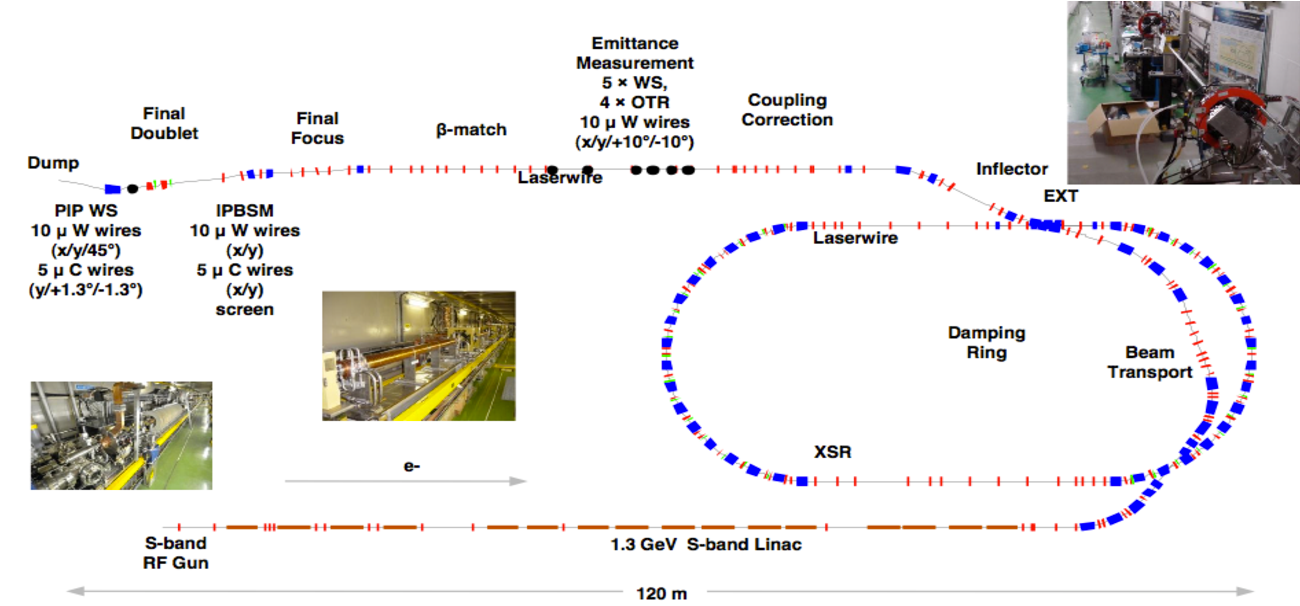
\includegraphics[angle=0,scale=0.70]{ATF-crop.pdf}\caption{Disposition of the Accelerator Test Facility (ATF), composed by a photocathode, a linac to 1.3GeV, a damping ring, an extraction line, the Final Focus (FF), and the beam dump.}\label{f:ATF_ATF2}
\end{subfigure}
\begin{subfigure}[b]{1.0\textwidth}
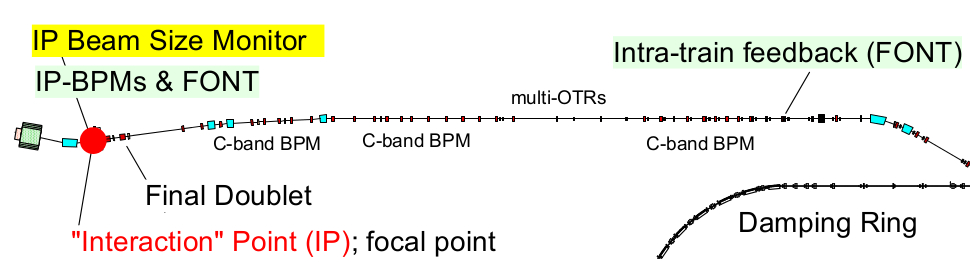
\includegraphics[angle=0,scale=0.65]{LigneATF2.jpg}\caption{Zoom over the extraction line, and Final Focus Section, highlighting the nominal Interaction Point location (IP). This region is known as ATF2.}\label{f:ATF2layout}
\end{subfigure}\caption{Diagrams containing the ATF composition and a zoom on the ATF2 section.}\label{f:ATF}
\end{figure}
\subsection{The RF Gun and Linac}
The total length of the linac is 80 m divided in: 18~m for the pre-injector section, a 70~m long accelerator section with energy compensation structures and 12~m for the transport line to the damping ring (DR) and a positron test stand.
The RF gun with a 1.6 cell S-Band Cs$_2$Te photocathode generates an electron beam with intensity up to 3.2nC per bunch. The pre-injector contains also an accelerating structure. An accelerating field of 35.2 MeV/m is required to accelerate 20 bunches of $2\times10^{10}$ particles per bunch. The linac is operated at a repetition rate of 25 pps (pulses per second) to allow circulating 5 bunch trains in the Damping ring. Table \ref{t:linac} shows the main parameters of the DR.
\begin{table}[hbt]
\centering
 \begin{tabular}{|c|c|}\hline
 Beam energy, $E_{beam}$& 1.54 GeV \\
 Bunch population, $N$& $2\times10^{10}$ \\
 Bunches per train, $N_b$ & 20 \\
 Bunch spacing, $\Delta t_{bunch}$ & 2.8 ns\\
 Energy spread Full Width, $\sigma_\delta$ & <1.0\% (90\% beam)\\
 Normalized emittance, $\epsilon_{Nx/y}$ & $< 3\times 10^{-4}$ m$\cdot$rad\\\hline
 \end{tabular}
 \caption{Basic design parameters of the ATF injector linac.}\label{t:linac}
\end{table}
\subsection{The Damping Ring}
The ring has a length of 138.6~m. It has achieved in 2004 a vertical normalized emittance of $1.5\times10^{-8}$ m$\cdot$rad, equivalent to $6$pm$\cdot$rad for a bunch intensity of $10^{10}$ particles. It was achieved by a precise alignment of components and beam control. The structure is a combination of bending magnets and wiggler cells where the value of the horizontal emittance is determined by the structure unit cell. The wigglers reduce the damping time and each bend is placed at the minimum of the dispersion in each periodic structure. The ATF DR consists in 36 of these units cells and the main parameters are in Table \ref{t:ATFDR}.
\begin{table}[hbt]
\centering
 \begin{tabular}{|c|c|}\hline
 Beam energy, $E_{beam}$& 1.54 GeV \\
 Bunch population, $N$& $2\times10^{10}$ \\
 Bunches per train, $N_b$ & 20 \\
 Bunch spacing, $\Delta t_{bunch}$ & 2.8 ns\\
 Energy spread Full Width, $\sigma_\delta$ & <1.0\% (90\% beam)\\
 Normalized emittance, $\epsilon_{Nx/y}$ & $3\times 10^{-6}/3\times 10^{-8}$ m$\cdot$rad\\\hline 
 \end{tabular}\caption{ATF DR main parameters.}\label{t:ATFDR}
\end{table}
\subsection{The extraction line}
In the extraction line the beam is extracted from the DR by means of a first kicker (KICKER1), and then passes off-axis through two quadrupoles centered on the DR reference orbit. Then, the beam passes through three septum magnets which complete the extraction. After the extraction, the beam passes through a dispersion supressor section to reduce fluctuations.\par
There are two extraction modes: single bunch and multibunch.\par
In single bunch mode one bunch is extracted approximately every 1/3 s from the damping ring to the ATF2 line. In multibunch mode a train of up to 20 bunches is extracted from the damping ring. The number of bunches and spacing are set by the damping ring fill up.\par
\subsection{The extraction diagnostic section}
After the extraction, the diagnostic section is used for measuring the emittance and dispersion ,and correcting betatron coupling. This section has been designed to be as close as possible to the ideal skew correction described in \cite{Woodley:453645}.\par
The measured vertical emittance in the diagnostic region downstream shows typically a factor 3~increase with respect to values obtained in the DR and dependence with beam intensity. One of the possibilities of the emittance growth is the non-linearity of the magnetic fields in the extraction region experienced by the beam when passing off-axis. One second possibility is the wakefields induced by the extraction kicker. The correlation with beam intensity is not fully understood; it could be due to the beam position monitors response.\par
Connecting dispersion and betatron matching plus careful alignment are the keys to mitigate the factor~3 increase in vertical emittance.\par
\subsection{The ATF2 lattice}
The ATF2 lattice can be subdivided in two sections : the matching section and the FFS. The following section describes the FFS.\par
% \subsubsection{The FFS}
The FFS focuses the beam to a small vertical beam size following the telescope design with local chromaticity correction, as in Sect. \ref{s:chromcorr}. The top of Fig.~\ref{f:FF_MADX} shows the lattice elements and the optics functions along the FFS. The Final Doublet (FD), QD0FF and QF1FF, provide the vertical and horizontal focusing, respectively. The horizontal off-momentum function $\eta$ and the pair of sextupoles in the FD are used to cancel the beam size dependence on energy spread at the IP.\par The second pair of sextupoles in the lattice section from 70~to~75~m are used to cancel the geometrical components induced by the sextupoles in the FD. And, additional chromaticity is created upstream QF7 to match the local correction~\cite{Raimondi:2000}, see Section \ref{s:chromcorr}.\par
\begin{figure}[htb]
 \vspace*{-1.5cm}
 \begin{picture}(0,0)
 \put(386,-76){\tiny IP}
 \put(372,-44){\tiny QD0}
 \put(354,-44){\tiny QF1}
 \put(198,-44){\tiny QF7}
%  \put(195,-43){\tiny IM}
%  \put(365,-76){\scriptsize FD}
 \put(70,-76){\scriptsize Matching Section}
 \put(220,-76){\scriptsize Final Focus Section (FFS)}
 \put(138,-286){\tikz\draw[blue,dashed,thick] (0,0) -- (0,8.42);}
%  \put(220,-30){\tikz\draw[red,dashed,thick] (0,0) circle (0.4);}
%  \put(-90,20){\hbar}
\end{picture}
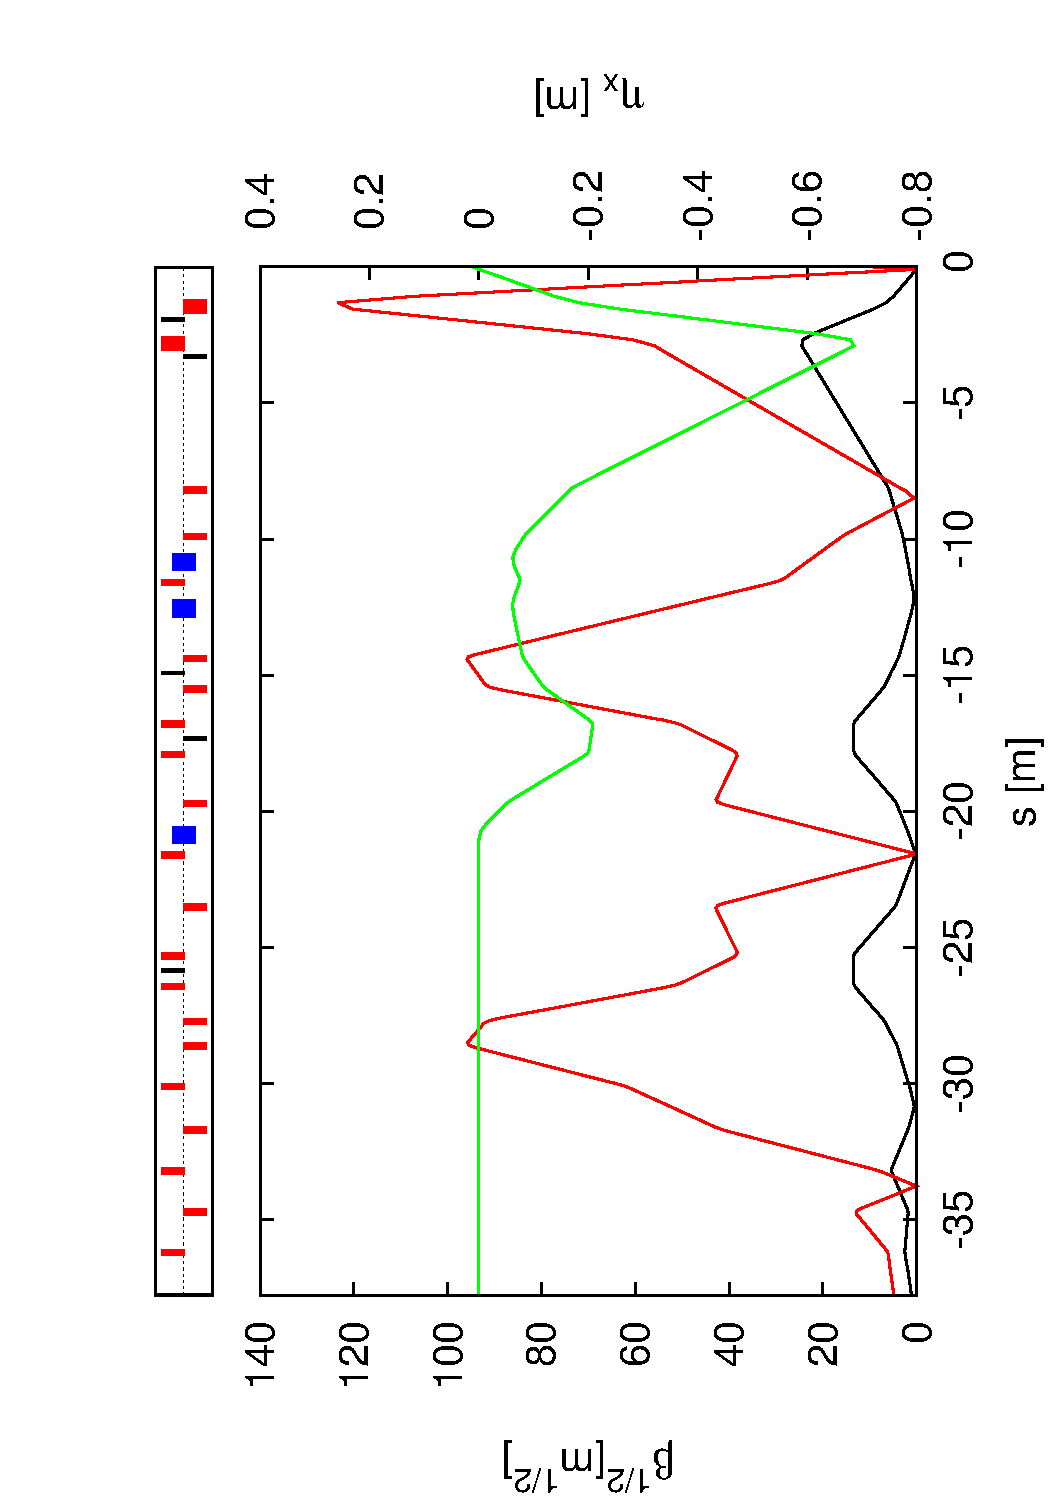
\includegraphics[angle=-90,scale=0.65]{lattice_ATF2_FF.pdf}\caption{Optical functions in the Final Focus Section at ATF2. On top is the ATF2 lattice: dipoles in blue, quadrupoles in red and sextupoles in black.}\label{f:FF_MADX}
\end{figure}
Quadrupole displacements are used to steer the beam, while sextupole displacements are used to induce corrective focusing (normal and skew components for horizontal and vertical displacements, respectively). This has an impact on the beam size. The tolerances to misalignments, roll angle and magnet strength errors in the FFS have been initially studied with a target of 2\% impact on the beam size, and it has resulted in similar tolerances as in ILC \cite{Yves}. 
All quadrupoles and sextupoles are placed on individual movers to allow the beam steering and adjustment of relative alignment in X, Y and Roll angle. 
\subsection{The IP Region}\label{s:opticsIP}
The $\beta$ functions at the IP, $\beta^*$, can be set by changing the matching section quadrupole strengths. Three configurations are normally used : 1BX1BY, 10BX1BY, and 100BX1000BY, where the factor indicates the number of times that the original $\beta^*$ has been amplified.\par
The 1BX1BY optics has the original design parameters. Here the angular divergence of the beam is $0.35$~mrad vertically and $0.52$~mrad horizontally in the IP region. \par
The 10BX1BY preserves the $\beta_y^*$ goal while relaxing the tolerance to multipole errors in magnets by increasing ten times the original $\beta_x^*$, making them comparable with those of ILC 500~GeV \cite{PhysRevSTAB.17.023501}. This optics is the one shown in Fig.~\ref{f:FF_MADX} and it is currently used in operation.\par
The 100BX1000BY optics sets a parallel beam through the IP area by enlarging the beam size at the IP. It is principally used to avoid the issues of large angle divergence displayed by the 1BX1BY optics.\par
Even smaller $\beta_y^*$ functions have been explored recently at ATF2 aiming to investigate resulting increases in tuning difficulty and beam size measurements limitations \cite{PateckiLowBeta}.\par
Figure \ref{f:BXYoptics} shows the beam size in vertical and horizontal planes for several optics combinations in a region of 300~mm around the IP. It also shows clearly how the beam divergence affects the beam size along the IP region.\par 
\begin{figure}[h]
 \begin{center}
 \hspace*{-1cm}
 \begin{subfigure}[b]{0.45\textwidth}
  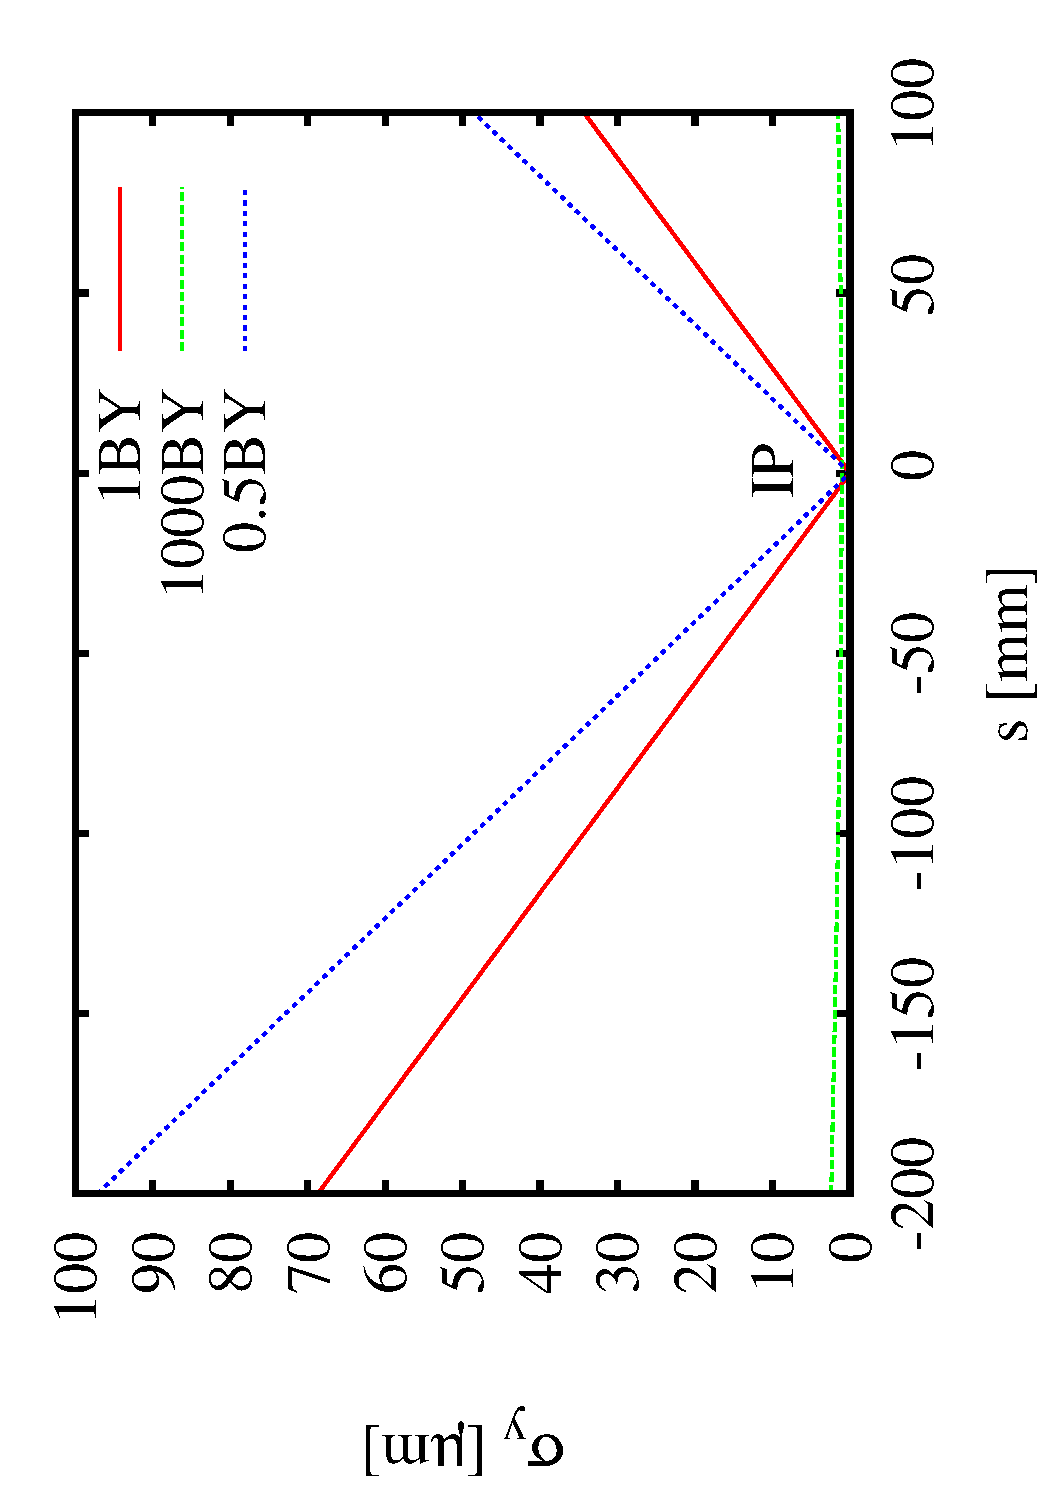
\includegraphics[angle=-90,scale=0.32]{optics_requ.pdf}\caption{Vertical beam size near the IP.}\label{f:opticsBY}
 \end{subfigure}\hspace{0.5cm}
\begin{subfigure}[b]{0.45\textwidth}
  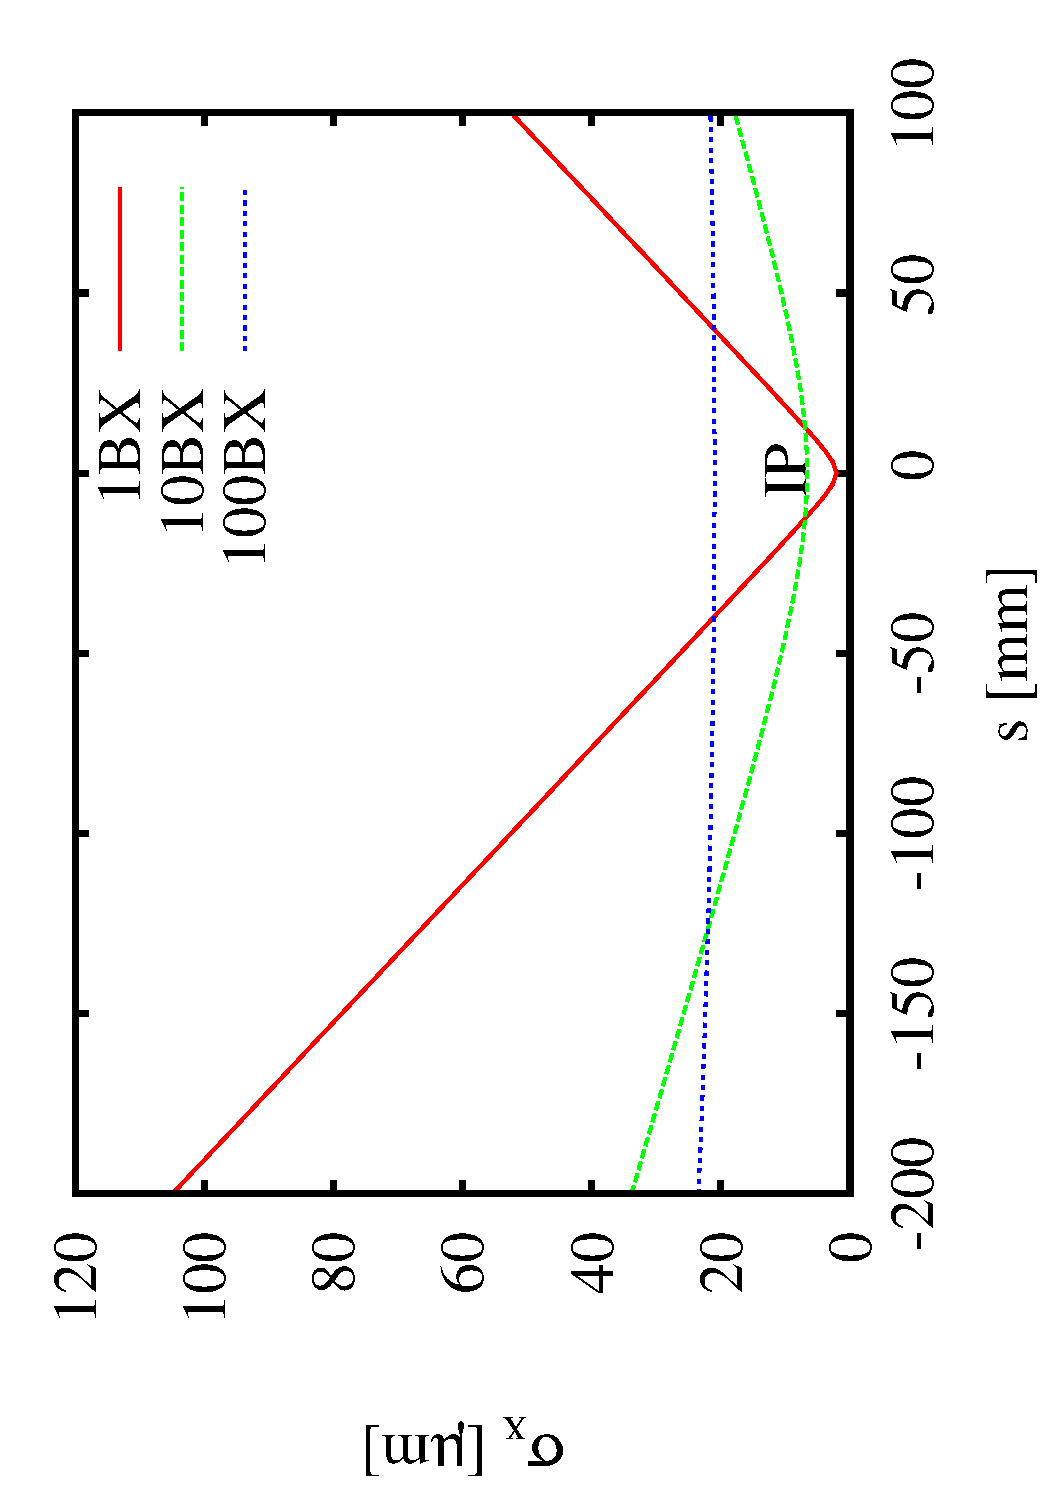
\includegraphics[angle=-90,scale=0.32]{optics_BX.pdf}\caption{Horizontal beam size near the IP.}\label{f:opticsBX}
 \end{subfigure}
  \caption{Vertical and horizontal beam sizes for 1BY, 1000BY, and 0.5BY in the vertical plane, and 1BX, 10BX and 100BX in the horizontal plane.}\label{f:BXYoptics}
 \end{center}
\end{figure}
The QD0 strength sets the vertical beam waist location with an small impact on the horizontal beam waist location, and viceversa for the QF1. The two are set to put the beam waist to its the nominal location at $s=0$. However, one or a combination of the two quadrupole strengths can be used to bring the beam waist to any location upstream or downstream. Moving the beam waist along the section of the IP region displayed in Fig.~\ref{f:BXYoptics} is effectively changing the focal distance by less than -20\% to +10\%.\par
QD0 and QF1 horizontal and vertical movers can also be used to steer the beam in the FD region, changing the position and angle through the IP region. Angles can also be steered by moving QF7 horizontally and vertically because of its location near a focal point upstream. See Fig. \ref{f:ATF2layout} showing the QF7 location and Eq. (\ref{eq:telescope}) to see that the kick at the input of a telescope lattice affects only the angle at the output.\par

\section{Beam Size Measurement at the IP}
A direct beam size measurement at the ATF2 IP is required because it can not be deduced from beam-beam effects as in a collider.\par
\begin{figure}[htb]
 \begin{center}
  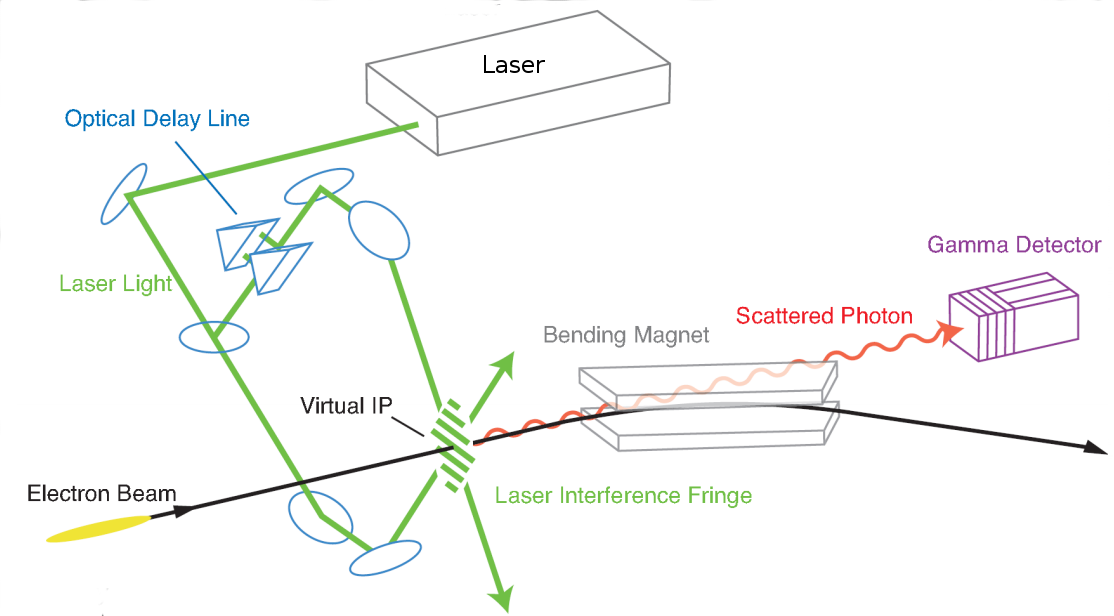
\includegraphics[angle=0,scale=0.5]{IPBSM_1.png}\caption{IPBSM schematic design. The particle beams cross the interference pattern generated by a perpendicular laser beam. The number of electron-photon interactions varies with the fringe size and the particle beam size.}\label{f:IPBSM}
 \end{center}
\end{figure}
The Beam Size Monitor (IPBSM) measures the number of scattered photons from an electron-photon collision between the particle bunch and a perpendicular interference pattern generated by high intensity laser perpendicular to the bunch trajectory \cite{Shintake1992453}. The number of photons is proportional to the photon density at the beam position. Moving the beam or scanning the phase of the laser fringe produces a modulation of gamma flux ray, the amplitude of which depends on beam size \cite{Yves}. Figure \ref{f:IPBSM} shows a schematic design of the IPBSM.\par
Such a device was previously used at the FFTB line at SLAC \cite{Shintake:1995sg}. A similar one is now located in the IP region at ATF2 \cite{Jackelinethese}.\par
\begin{figure}[htb]
 \begin{center}
  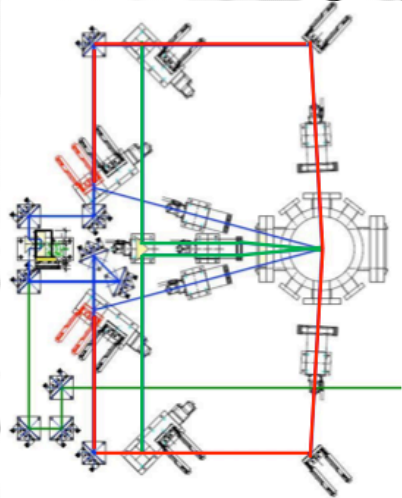
\includegraphics[angle=0,scale=0.35]{IPBSM_angles.png}
  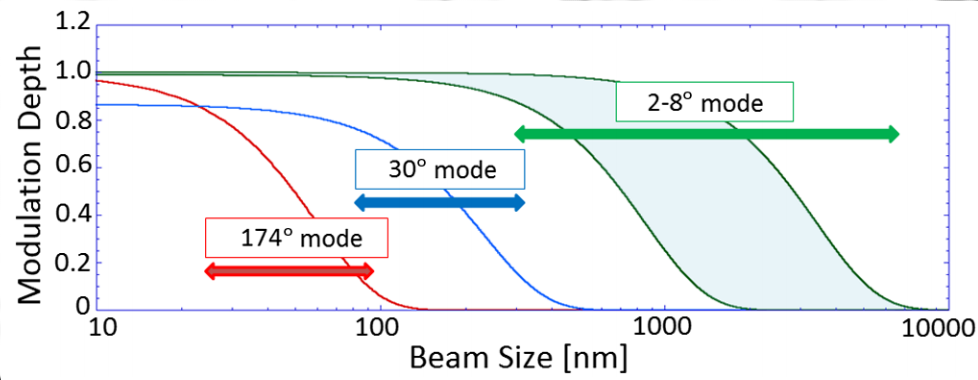
\includegraphics[angle=0,scale=0.455]{IPBSMreso.png}
  \caption{(Right) IPBSM laser path over the optical table perpendicular to the beam propagation. (Left) Beam size resolution for the angle modes : $2\sim8$\degree in green, 30\degree in blue and 174\degree in red.}\label{f:IPBSMangles}
 \end{center}
\end{figure}
At ATF2, it is installed on a vertical optical table where the laser incident angle can be adjusted to change the interference fringe pitch allowing measurements of beam sizes from 6~$\mu$m down to 25~nm. Figure \ref{f:IPBSMangles} shows the laser beam paths along the vertical optical table for three angle modes and the corresponding ranges of possible beam measurements.\par
Larger beam sizes are measured by a wire scanner installed in the same region. It consists in a wire moved across the beam generating bremsstrahlung gamma rays. The number of photons is proportional to the charge of the slice interacting with the wire at each position setting. Profiles are constructed from the number of photons as a function of wire position \cite{Hayano:2000xf}.

\section{Beam stabilization}
Three regimes are defined for the beam stability: random fluctuations over timescales which are effectively uncorrectable (jitter), fast varitions that can be corrected by feedback (FB) systems, and slow or static changes that can be addressed by systematic orbit correction (tuning).\par
The jitter requirement for goal 1 is beam jitter less than 30\% of $\sigma_y$, while goal 2 requires jitter less than 5\% of $\sigma_y$. The measured bunch position jitter upstream of the FD for single bunch extraction mode, i.e. the fluctuations on bunch position before the last strong focusing magnets, is around 10$\sim$20\% of beam size in the vertical plane and 5$\sim$10\% on the horizontal plane \cite{PateckiJitter}. Additional jitter could come from the mechanical vibration of the FD.\par
\subsection{Tuning}
The contribution to beam size due to field errors is considered static or slowly changing. It is possible to reduce their impact by systematic orbit correction using magnetic or mechanical means~\cite{ATF2prop}. Goal 1 jitter requirements can be achieved for single bunch extraction.\par
\subsection{Feedback}
The fluctuations coming from ground motion, magnet strength variations, changes in the damping ring, energy oscillations are considered fast errors. Aso, the bunch to bunch jitter from multibunch extraction requires active correction.\par 
The feedback system is then the last line of defense to correct the beam trajectory and three schemes are tested in ATF2 using two bunches.\par
\begin{itemize}
 \item Upstream FB: Measures the first bunch position in the IP region and uses a set of kickers upstream of the matching section to stabilize the position of the second bunch.
 \item Feedforward: Measures the first bunch position upstream of the matching section and uses a kicker in the IP region to stabilize the position of a second.
 \item Local IP FB: Measures the first bunch position in the IP region and uses a kicker in the IP region to stabilize the position of a second.
\end{itemize}

\section{Recent achievements and current work}
In 2014 vertical beam size about 55~nm was observed at ATF2 \cite{Kubo50nm}, and since then smaller beam size are achieved as a regular basis down to 44~nm \cite{KuboCLICws2015}, demonstrating the local chromaticity correction method at charges of about~$0.1\times10^{10}$ particules per bunch.\par
A main identified issue, intensity dependence, is currently explored by the ATF2 collaboration. Nonetheless, at low intensities, the beam size remains above the design 37~nm. Possible contributions are: (1) the increase of the incoming beam emittance along the ATF2 line, (2) systematic errors and resolution limitations on the beam size monitor, (3) beam drift/jitter beyond the tolerable margin and  (4) undetected optics mismatch.\par
Last two issues can be adressed by measuring the beam trajectory in the IP Region after the Final Doublet. In addition, looking forward to \textbf{goal 2}, beam position measurement is a requirement for beam stabilization.\par
The work here described corresponds to the beam position monitors installed in 2013 by LAL in collaboration with Kyungpook National University (KNU), the Feedback in Nanosecond Timescale (FONT) group from Oxford, and the ATF2 staff.\par

\section{Position Measurement Requirements}
A direct beam position measurement at the ATF2 IP is required because it can~not be deduced from beam-beam focusing effects as in a collider \cite{Bambade:1989pb}.\par
Knowing the beam trajectory with nanometric precision is valuable information for beam tuning and a requirement for feedback. The position measurement system could be used to correct the beam positions used in the reconstruction of the IPBSM modulation pattern, in order to remove the dilution from beam jitter in the beam size reconstruction pulse by pulse.\par
Therefore, a set of three cavities (IPA, IPB and IPC), two upstream and one downstream of the nominal IP, were installed and are used to measure the beam trajectory in the IP region, thus providing enough information to reconstruct the bunch position and angle at the IP.\par
Cavities are located at $s=-167.9$ mm, $s=-87.1$ mm and $s=87.1$ mm, with respect to the nominal IP at $s=0$. It has been shown in section \ref{s:opticsIP} the effect of different optics on the beam size along the IP region. As the measured beam jitter upstream is around $10\sim20$\% of beam size, then, the change of optics will have a direct impact on the dynamic range of the position measurement.\par %The following subsections give an estimation of the beam jitter.\par
% \subsubsection{Beam waist at one cavity using 1BX1BY and 10BX1BY optics}
\subsubsection{Dynamic Range}
Table \ref{t:sigmacavities1000BY} shows that beam size only increases by a factor two among the cavities using the 1000BY optics, while Table \ref{t:sigmacavities1BY} shows a beam one and two thousand times larger than the beam size at the focal point, due to the large divergence in the nominal optics.\par
From these optics settings the maximum vertical beam size is 58~$\mu$m. The dynamic range required for the cavity is then around 10~to~11~$\mu$m using the 20\% jitter to beam size ratio.
\begin{table}[h]
 \centering
\begin{tabular}{c||c|c|c|c}\hline
  & IPA & IPB & IP & IPC\\\hline\hline
  $s$ [mm]& -174.2 & -87.1 & 0 & 87.1 \\\hline
  $\sigma_y$ [1.086$\mu$m]&2.0&1.3&1&1.3\\\hline
  $\sigma_{y'}[0.011$mrad]&0.5&0.8&1&0.8\\\hline
\end{tabular}\caption{Vertical beam size at the cavities positions and the IP with the 1000BY optics.}\label{t:sigmacavities1000BY}
\end{table}
\begin{table}[h]
 \centering
\begin{tabular}{c||c|c|c|c}\hline
  & IPA & IPB & IP & IPC\\\hline\hline
  $s$ [mm] & -174.2 & -87.1 & 0 & 87.1\\\hline
  $\sigma_y$ [34~nm]&$1.7\times10^3$&871&1&871\\\hline
  $\sigma_{y'}$ [0.3~mrad]&$0.6(10^{-3})$&$1.2(10^{-3})$&1&$1.2(10^{-3})$\\\hline
\end{tabular}\caption{Vertical beam size at the cavities positions and the IP with the 1BY optics.}\label{t:sigmacavities1BY}
\end{table}
\subsubsection{Resolution and Calibration}
The beam stabilization to the nanometer level requires position measurement with nanometric resolution. In addition, due to the low $\beta^*$ for the nominal 1BX1BY optics, the beam size and therefore the jitter increases rapidly making the 1~nm resolution over the 10~$\mu$m dynamic range a challenge. The calibrations must be then valid for measurement over 3 to 4 order of magnitude.\par
